% TeX encoding = utf8
% TeX spellcheck = pl_PL 
\documentclass[a4paper, 12pt]{article}
\usepackage[utf8]{inputenc}
\usepackage[polish]{babel}
\usepackage{polski}
\usepackage{graphicx}
\usepackage{listings}
\usepackage{amsfonts}
\usepackage{geometry}
\usepackage{indentfirst}
\usepackage{subfigure}
\usepackage{url}
\usepackage{listings}
\usepackage{color}
\usepackage[usenames,dvipsnames]{xcolor}

%\renewcommand*{\addcontentsline}[3]{\addtocontents{#1}{\protect\contentsline{#2}{#3}{}}}
%\newgeometry{tmargin=2.5cm, bmargin=2.5cm, lmargin=3.5cm, rmargin=2.5cm}
%\setcounter{secnumdepth}{2}
\setlength{\fboxsep}{0pt}
\lstset{
	basicstyle=\footnotesize\ttfamily,
	breaklines=true,
	language=Python,
	breakatwhitespace=true,
	frame=leftline,
	numbers=left,
	numberstyle=\tiny,
	commentstyle=\color{Gray}\footnotesize\ttfamily}


\author{Anna Wujek \\ Łukasz Korpal \\ Wiktor Ślęczka}
\title{Analiza zagadnienia i przygotowanie środowiska roboczego}

\begin{document}
	\sloppy
	\maketitle
	\section{Zadanie}
	Celem zadania jest stworzenie projekt oraz implementacji symulatora mobilnej sieci ad hoc (MANET) do monitorowania skażenia środowiska naturalnego. Węzłami sieci będą wyposażone w czujniki, komunikujące się między sobą roboty mobilne. Zadaniem sieci będzie lokalizacja chmury skażenia i otoczenie jej robotami, monitorującymi jej położenie i granice, przy założeniu utrzymania spójności.
	
	\subsection{Założenia}
	\begin{itemize}
		\item Roboty potrafią się na bieżąco lokalizować.
		\item System składa się z pewnej liczby robotów mobilnych oraz jednostki centralnej odbierającej od robotów dane o skażeniu.
		\item Roboty mobilne działają autonomicznie i potrafią same zorganizować sieć.
		\item Roboty są wyposażone w czujniki pozwalające im wykrywać poziom skażenia oraz przeszkody.
		\item Roboty są wyposażone w urządzenia pozwalające im na komunikację z pozostałymi robotami.
	\end{itemize}
	
	\subsection{Scenariusz działania}

		\textbf{Wariant z samoorganizacją}
		
		Nieznana jest mapa przestrzeni roboczej oraz lokalizacja chmury skażenia. Roboty są autonomiczne w zakresie omijania przeszkód, a także same organizują się w sieć, a do jednostki centralnej tylko wysyłają dane o skażeniu. Ważne jest w tym przypadku dbanie o zachowanie spójności sieci, zwłaszcza podczas omijania przeszkód. Chmura może się przemieszczać oraz zmieniać kształt w trakcie zadania. Roboty poszukują granic chmury oraz starają się ją całkowicie otoczyć.
		
		
	
	\subsection{Narzędzia}
	Wykorzystany zostanie symulator V-rep w połączeniu z językiem skryptowym Python. V-rep posłuży jako symulator środowiska oraz robotów i ich czujników, natomiast w języku Python zaimplementowana zostanie jednostka centralna oraz logika robotów.
	
	W ramach przygotowania środowiska stworzyliśmy niewielki program do sterowania robotem z zewnętrznego skryptu, który uruchamia silnik robota i odczytuje stan czujników. 
	
	\begin{figure}[h!]
	\centering
	\frame{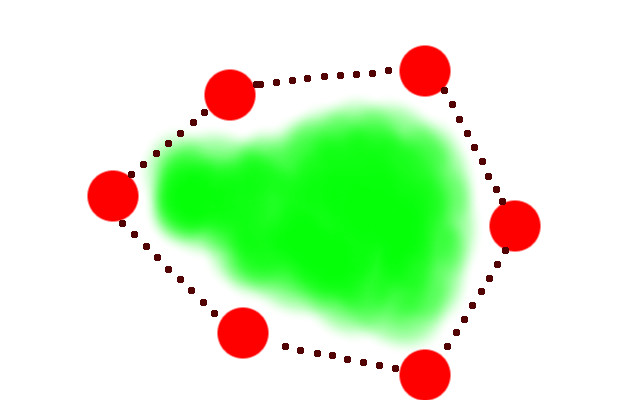
\includegraphics[width=0.7\columnwidth]{img/chmura.jpg}}
	\caption{Przykładowy sposób otoczenia chmury skażenia przez roboty.}
	\end{figure}
	


	
\end{document}


